% Originally: content/week-03.tex, \section{Connectedness} (Corsin Week 3, Monday)

\section{Connectedness}
\label{sec:connectedness}

\begin{definition}[Connected and disconnected metric spaces]
\label{def:connectedness}
A metric space $(X,d)$ is \newterm{disconnected} (\germanterm{unzusammenh\"angend}) if there
exist $U_1, U_2 \subseteq X$ subsets which are
\begin{enumerate}[label=\textbf{(\alph*)}]
  \item \textbf{open},
  \item \textbf{non-empty}, $U_1 \neq \emptyset \neq U_2$,
  \item \textbf{disjoint}, $U_1 \cap U_2 = \emptyset$,
\end{enumerate}
such that $X = U_1 \cup U_2$. Similarly, for a subset $A \subseteq X$, it is disconnected if it is
disconnected as a metric space with the induced metric $d|_{A \times A}$. \newterm{Connected}
(\germanterm{zusammenh\"angend}) is the negation of disconnected.
\end{definition}

Typically, proving that a set or metric space is connected is done \textbf{by contradiction},
which is why one should remember the definition of \textit{disconnected}. Intuitively, connected
means: \qt{the space cannot be separated by open sets.}

\begin{center}
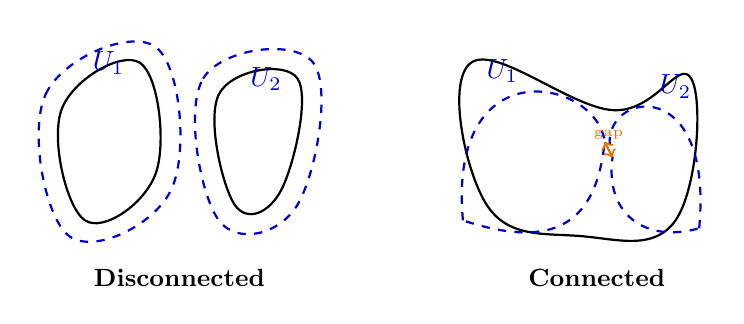
\begin{tikzpicture}[scale=1.0]
  % Left panel: Disconnected
  \begin{scope}[shift={(0,0)}]
    \draw[thick] plot[smooth cycle, tension=0.7] coordinates {(-1.5,-0.8) (-1.8,0.6) (-0.8,1.2) (-0.6,-0.2)};
    \draw[thick] plot[smooth cycle, tension=0.7] coordinates {(0.4,-0.6) (0.2,0.8) (1.2,1.0) (1.0,-0.4)};

    \draw[blue!80!black, thick, dashed] plot[smooth cycle, tension=0.7] coordinates {(-1.7,-1.0) (-2.0,0.8) (-0.6,1.4) (-0.4,-0.4)};
    \node[blue!80!black] at (-1.2,1.2) {$U_1$};

    \draw[blue!80!black, thick, dashed] plot[smooth cycle, tension=0.7] coordinates {(0.2,-0.8) (0.0,1.0) (1.4,1.2) (1.2,-0.6)};
    \node[blue!80!black] at (0.8,1.0) {$U_2$};

    \node[below, font=\small] at (-0.3,-1.3) {\textbf{Disconnected}};
  \end{scope}

  % Right panel: Connected
  \begin{scope}[shift={(5.0,0)}]
    \draw[thick] plot[smooth cycle, tension=0.7] coordinates {(-1.4,-0.6) (-1.6,1.2) (0.2,0.6) (1.2,1.0) (1.0,-0.8) (-0.2,-1.0)};

    \draw[blue!80!black, thick, dashed] (-1.7,-0.8).. controls (-1.9,1.4) and (0.0,1.0).. (0.1,0.2).. controls (0.0,-0.8) and (-0.5,-1.2).. (-1.7,-0.8);
    \node[blue!80!black] at (-1.2,1.1) {$U_1$};

    \draw[blue!80!black, thick, dashed] (1.3,-0.9).. controls (1.5,1.2) and (-0.1,0.8).. (0.2,0.0).. controls (0.1,-0.7) and (0.6,-1.1).. (1.3,-0.9);
    \node[blue!80!black] at (1.0,0.9) {$U_2$};

    \draw[orange!90!black, <->, thick] (0.1,0.2) -- node[above, font=\tiny] {gap} (0.2,0.0);

    \node[below, font=\small] at (0,-1.3) {\textbf{Connected}};
  \end{scope}
\end{tikzpicture}
\end{center}

% Generator: Claude Opus 5 (High) --- the base case of connectedness, used three times in this
% chapter (path-connectedness, the topologist's sine curve, the intermediate value theorem)
% but stated nowhere in the source notes.
\begin{proposition}[Intervals are connected]
\label{prop:intervals_connected}
Every interval $I \subseteq \mathbb{R}$ --- open, closed, half-open, bounded or not --- is
connected (\cref{def:connectedness}). Conversely, a connected subset of $\mathbb{R}$ is an
interval.
\end{proposition}

\begin{proof}
Suppose $I = U_1 \sqcup U_2$ with $U_1, U_2$ open in $I$, disjoint and both non-empty. Pick
$a \in U_1$ and $b \in U_2$; without loss of generality $a<b$, and $[a,b] \subseteq I$ because
$I$ is an interval. Set
\[c := \sup\{\,t \in [a,b] \ :\ [a,t] \subseteq U_1\,\},\]
which is well defined since $a$ belongs to the set. Now $c \in [a,b] \subseteq I$, so $c$ lies
in $U_1$ or in $U_2$, and both lead to a contradiction:
\begin{itemize}
  \item If $c \in U_1$, openness gives $\varepsilon>0$ with $(c-\varepsilon,c+\varepsilon)\cap I
    \subseteq U_1$; together with $[a,c) \subseteq U_1$ this yields $[a,t] \subseteq U_1$ for
    some $t>c$ unless $c=b$ --- contradicting either the supremum or $b \in U_2$.
  \item If $c \in U_2$, openness gives $\varepsilon>0$ with $(c-\varepsilon,c] \cap I \subseteq
    U_2$. But $c>a$ (as $a \in U_1$ is open in $I$), so by definition of the supremum there is
    $t \in (c-\varepsilon,c]$ with $[a,t] \subseteq U_1$ --- contradicting disjointness.
\end{itemize}
So no such splitting exists, and $I$ is connected. For the converse, a set $A \subseteq
\mathbb{R}$ that is not an interval admits $a<c<b$ with $a,b \in A$ and $c \notin A$; then
$A \cap (-\infty,c)$ and $A \cap (c,\infty)$ disconnect it.
\end{proof}

\begin{remark}[Why this is the only example one ever needs]
\label{rem:intervals_are_the_base_case}
Every connectedness proof in this chapter reduces to \cref{prop:intervals_connected}: a path is
a continuous image of $[0,1]$ (\cref{def:path}), so path-connected sets are connected
(\cref{lem:path_connected_implies_connected}) purely because the \emph{interval} is; and the
intermediate value theorem, invoked in the topologist's sine curve below, is
\cref{thm:continuity_preserves_connected} applied to an interval, since the connected subsets of
$\mathbb{R}$ are exactly the intervals. In other words, the single fact that $\mathbb{R}$ has no
gaps --- the completeness axiom, which is what powers the supremum above --- is the source of
all of it.
\end{remark}

\begin{aiexample}[Disconnectedness of Rational Numbers]
% Generator: Gemini 3.6 Flash (Medium)
The set of rational numbers $\mathbb{Q} \subset \mathbb{R}$ equipped with the subspace topology is disconnected. To see this, define
\[
U := \mathbb{Q} \cap (-\infty, \sqrt{2}) \quad \text{and} \quad V := \mathbb{Q} \cap (\sqrt{2}, \infty).
\]
Since $\sqrt{2} \notin \mathbb{Q}$, we have $U \cup V = \mathbb{Q}$ and $U \cap V = \emptyset$. Both $U$ and $V$ are non-empty and open in the subspace topology of $\mathbb{Q}$ (as intersections of $\mathbb{Q}$ with open intervals in $\mathbb{R}$). Hence $U$ and $V$ form a separation of $\mathbb{Q}$.
\end{aiexample}

% Supplement: Sascha Brack/Class Notes/Week_02_Notes_Friday_Updated.pdf, p. 9
\begin{example}[A disconnected set in $\mathbb{R}^2$]
Let $X := ([0,1] \times [0,1]) \cup ([2,3] \times \{1\}) \subseteq \mathbb{R}^2$. Is $X$ connected?
No. Let $U := \{(x,y) \in X \mid x < 1.5\}$ and $V := \{(x,y) \in X \mid x > 1.5\}$. We can write these as $U = X \cap \{(x,y) \in \mathbb{R}^2 \mid x < 1.5\}$ and $V = X \cap \{(x,y) \in \mathbb{R}^2 \mid x > 1.5\}$. Both $U$ and $V$ are open in the subspace topology of $X$ because they are intersections of $X$ with open half-planes in $\mathbb{R}^2$. Furthermore, $X = U \cup V$, and $U, V$ are disjoint and non-empty. Thus, $X$ is disconnected.
\begin{center}
\begin{tikzpicture}[scale=1.5]
  \draw[->, thick] (-0.2,0) -- (3.5,0);
  \draw[->, thick] (0,-0.2) -- (0,1.5);
  
  \draw[very thick, fill=purple!20, pattern=north east lines, pattern color=purple] (0,0) rectangle (1,1);
  \draw[very thick, purple] (2,1) -- (3,1);
  \node[purple, left] at (-0.1, 0.5) {$X$};
  
  \draw[green!60!black, dashed] (0.5, 0.5) circle (0.8);
  \node[green!60!black] at (1.2, 0.6) {$U$};
  
  \draw[green!60!black, dashed] (2.5, 1) ellipse (0.7 and 0.3);
  \node[green!60!black] at (2.5, 1.4) {$V$};
\end{tikzpicture}
\end{center}
\end{example}

\begin{theorem}[Continuous functions preserve connectedness]
\label{thm:continuity_preserves_connected}
Let $X$, $Y$ be metric spaces, $f : X \to Y$ continuous. If $A \subseteq X$ is connected, then
$f(A)$ is connected.
\end{theorem}

% Generator: Claude Opus 5 (High) --- stated without proof in the source; the argument is three
% lines and is the exact dual of \cref{item:continuity_preserves_compact}.
\begin{proof}
We may assume $A = X$, replacing $X$ by $A$ with the induced metric and $Y$ by $f(A)$. Suppose
$f(X)$ were disconnected, say $f(X) = V_1 \sqcup V_2$ with $V_1,V_2$ open in $f(X)$, disjoint
and non-empty. Then $U_i := f^{-1}(V_i)$ is open by \cref{def:continuous}\textbf{(c)},
non-empty because $V_i$ meets the image, and $U_1 \cap U_2 = \emptyset$ with
$U_1 \cup U_2 = X$ because the $V_i$ partition $f(X)$. So $U_1,U_2$ disconnect $X$, contrary to
hypothesis.
\end{proof}

\begin{corollary}[Intermediate value theorem]
\label{cor:intermediate_value_theorem}
Let $f : [a,b] \to \mathbb{R}$ be continuous. Then $f$ attains every value between $f(a)$ and
$f(b)$.
\end{corollary}

\begin{proof}
By \cref{prop:intervals_connected}, $[a,b]$ is connected, so $f([a,b])$ is connected by
\cref{thm:continuity_preserves_connected}, hence is an interval (\cref{prop:intervals_connected}
again). An interval containing $f(a)$ and $f(b)$ contains everything between them.
\end{proof}

\begin{ainote}
The intermediate value theorem is a result from \emph{Analysis I}, but it is worth re-deriving
it here in one line: it is the first place where connectedness earns its keep, and the proof
makes visible that the theorem is really a statement about $\mathbb{R}$ having no gaps rather
than about $f$. It is used in the topologist's sine curve
(\cpageref{ex:topologists_sine_curve}) below.
\end{ainote}

% Supplement: Sascha Brack/Class Notes/Week_03_Notes_Monday.pdf, p. 4
\begin{corollary}[Linear maps preserve the unit cube]
\label{cor:linear_maps_unit_cube}
Given the $n$-dimensional unit cube $[0,1]^n \subset \mathbb{R}^n$, any linear map $L : \mathbb{R}^n \to \mathbb{R}^n$ maps $[0,1]^n$ to an $n$-dimensional parallelepiped. Since linear maps in Euclidean space are continuous, the image $L([0,1]^n)$ is connected. Furthermore, since $[0,1]^n$ is compact, $L([0,1]^n)$ is also compact.
\end{corollary}

\begin{exercise}[Properties of connectedness]
\label{ex:connectedness_tf}
Are the following true or false?
\begin{enumerate}[label=\textbf{(\alph*)}]
  \item The union of connected subsets with a common point is connected.
  \item The intersection of connected subsets is connected.
  % Not a first introduction -- \newterm/\germanterm for "closure" belong to
  % \cref{def:interior_closure_boundary}, so this is a plain back-reference.
  \item The closure (\cref{def:interior_closure_boundary}) of a connected subset is connected.
\end{enumerate}
\end{exercise}

% Kept inline: solved directly in Corsin Nick/Class Notes/Week 3.pdf, pp. 5--6.
\begin{exercisesolution}[Proof of \cref{ex:connectedness_tf}]
\textbf{(a) True.} \textit{Proof.} Let $X$ be a metric space, $V_1, V_2 \subseteq X$ connected,
and $x_0 \in V_1 \cap V_2$. Suppose $V_1 \cup V_2 \subseteq U_1 \cup U_2$ with
$U_1, U_2 \subseteq X$ open and disjoint. Assume without loss of generality $x_0 \in U_1$. Then
$U_1 \cap V_1 \neq \emptyset$ and $U_1 \cap V_2 \neq \emptyset$. So, since $V_1, V_2$ are
connected, $V_1 \cap U_2 = V_2 \cap U_2 = \emptyset$. Therefore
$(V_1 \cup V_2) \cap U_2 = \emptyset$ and $V_1 \cup V_2$ is connected.

\textbf{(b) False.} \textit{Counterexample:}
\[
X = \mathbb{R}^2, \quad U = [-1,1] \times \{0\}, \quad V = S^1 = \{x \in \mathbb{R}^2 : \|x\| = 1\},
\]
\[
U \cap V = \{(-1,0), (1,0)\}.
\]

\textbf{(c) True.} Suppose $X$ is a metric space, $A \subseteq X$ a subset with closure
$\overline{A}$. Suppose $U_1, U_2 \subseteq X$ are disjoint open sets covering $\overline{A}$, and
assume without loss of generality $\overline{A} \cap U_1 \neq \emptyset$. Then, since $U_1$ is
open, $A \cap U_1 \neq \emptyset$. By connectedness of $A$, $U_2 \cap A = \emptyset$, and since
$U_2$ is open, also $U_2 \cap \overline{A} = \emptyset$.
\end{exercisesolution}

\begin{ainote}
Corsin writes $\|x\| = R^2$ in the definition of $S^1$ above; it must be $\|x\| = 1$, as the
stated intersection $\{(\pm 1, 0)\}$ confirms. Corrected here.
\end{ainote}

\begin{center}
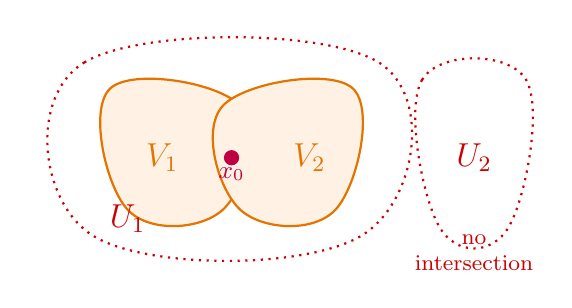
\begin{tikzpicture}[scale=1.1]
  \draw[orange!90!black, thick, fill=orange!10] plot[smooth cycle, tension=0.7] coordinates {(-1.6,-0.6) (-1.8,0.8) (-0.3,0.6) (-0.5,-0.6)};
  \node[orange!90!black, font=\large] at (-1.2,0) {$V_1$};

  \draw[orange!90!black, thick, fill=orange!10] plot[smooth cycle, tension=0.7] coordinates {(-0.3,-0.6) (-0.5,0.6) (1.0,0.8) (0.8,-0.6)};
  \node[orange!90!black, font=\large] at (0.5,0) {$V_2$};

  \fill[purple] (-0.4,0) circle (2.5pt) node[below, font=\small] {$x_0$};

  \draw[red!80!black, thick, dotted] plot[smooth cycle, tension=0.7] coordinates {(-2.0,-0.9) (-2.1,1.1) (1.3,1.1) (1.1,-0.9)};
  \node[red!80!black, font=\large] at (-1.6,-0.7) {$U_1$};

  \draw[red!80!black, thick, dotted] plot[smooth cycle, tension=0.7] coordinates {(2.0,-0.8) (1.8,0.9) (3.0,0.9) (2.8,-0.8)};
  \node[red!80!black, font=\large] at (2.4,0) {$U_2$};
  \node[red!80!black, font=\footnotesize, align=center] at (2.4,-1.1) {no\\intersection};
\end{tikzpicture}
\end{center}

\begin{center}
\begin{tikzpicture}[>=Latex, scale=1.3]
  \draw[->] (-1.6,0) -- (1.6,0) node[right] {$x$};
  \draw[->] (0,-1.6) -- (0,1.6) node[above] {$y$};

  \draw[red!80!black, thick] (0,0) circle (1.0);
  \node[red!80!black, above right] at (0.7,0.7) {$S^1$};

  \draw[orange!90!black, ultra thick] (-1,0) -- (1,0);
  \node[orange!90!black, below] at (0,-0.1) {$U = [-1,1]\times\{0\}$};

  \fill[purple] (-1,0) circle (2pt) node[above left, font=\footnotesize] {$(-1,0)$};
  \fill[purple] (1,0) circle (2pt) node[above right, font=\footnotesize] {$(1,0)$};
\end{tikzpicture}
\end{center}
